% ============================================================================
% FL-EHDS Paper for FLICS 2026
% IEEE Conference Format - IMPROVED VERSION
% Version: 2.0 - February 2026
% ============================================================================

\documentclass[conference]{IEEEtran}

% ===== PACKAGES =====
\usepackage{cite}
\usepackage{amsmath,amssymb,amsfonts}
\usepackage{graphicx}
\usepackage{textcomp}
\usepackage{xcolor}
\usepackage{booktabs}
\usepackage{hyperref}
\usepackage{url}

% TikZ for vector figures
\usepackage{tikz}
\usetikzlibrary{shapes.geometric, arrows.meta, positioning, fit, backgrounds, calc}

% ===== DOCUMENT =====
\begin{document}

\title{FL-EHDS: A Privacy-Preserving Federated Learning Framework for the European Health Data Space}

\author{
    \IEEEauthorblockN{Fabio Liberti}
    \IEEEauthorblockA{
        Department of Computer Science\\
        Universitas Mercatorum, Rome, Italy\\
        fabio.liberti@unimercatorum.it\\
        ORCID: 0000-0000-0000-0000
    }
}

\maketitle

% ============================================================================
% ABSTRACT
% ============================================================================
\begin{abstract}
The European Health Data Space (EHDS), established by Regulation (EU) 2025/327 and effective March 2025, mandates cross-border health data analytics while preserving citizen privacy. Federated Learning (FL) emerges as the key enabling technology for secondary use, yet systematic evidence synthesis reveals critical implementation gaps: only 23\% of FL implementations achieve sustained production deployment in healthcare settings, with hardware heterogeneity (78\%) and non-IID data distributions (67\%) as dominant technical barriers. Legal uncertainties regarding gradient data status under GDPR and controller/processor responsibilities remain unresolved. We present FL-EHDS, a three-layer compliance framework integrating governance mechanisms (Health Data Access Bodies, data permits, opt-out registries), FL orchestration (aggregation within Secure Processing Environments, differential privacy), and data holder components (adaptive training, FHIR preprocessing). The framework maps evidence-based barriers to specific mitigation strategies and provides compliance checkpoints aligned with EHDS requirements. This paper contributes: (1) the first systematic barrier taxonomy for FL in EHDS contexts based on 47 documents following PRISMA methodology; (2) a reference architecture addressing identified technical, legal, and organizational gaps; (3) an implementation roadmap for the critical 2025-2031 transition period with prioritized actions for policymakers, national authorities, and healthcare organizations.
\end{abstract}

\begin{IEEEkeywords}
Federated Learning, European Health Data Space, Privacy-Preserving Technologies, GDPR, Health Data Governance, Cross-Border Analytics, Differential Privacy
\end{IEEEkeywords}

% ============================================================================
% 1. INTRODUCTION
% ============================================================================
\section{Introduction}
\label{sec:introduction}

The European Health Data Space (EHDS), established by Regulation (EU) 2025/327, represents the European Union's most ambitious initiative for cross-border health data governance~\cite{eu2025ehds}. Entering into force on 26 March 2025, the regulation creates a dual framework: primary use through MyHealth@EU infrastructure for direct patient care, and secondary use through HealthData@EU for research, innovation, and evidence-based policy-making~\cite{hussein2025interop}.

The EHDS introduces novel governance mechanisms of unprecedented complexity. Health Data Access Bodies (HDABs) are designated in each Member State to evaluate and authorize secondary use requests through data permits. Article 53 enumerates permitted purposes including scientific research, public health surveillance, and AI training; Article 71 introduces opt-out mechanisms allowing citizens to object to secondary use of their electronic health data~\cite{staunton2024ethical}. The implementation timeline extends to 2031, with delegated acts expected by March 2027 and secondary use provisions applicable from March 2029.

\subsection{The Technology-Governance Divide}

Federated Learning (FL) emerges as the theoretically ideal technical solution for EHDS secondary use---the model travels to distributed data sources rather than centralizing sensitive health records~\cite{rieke2020future}. This ``data stays home'' principle aligns with GDPR data minimization requirements and addresses legitimate concerns about health data sovereignty across 27 Member States~\cite{mcmahan2017communication}.

However, recent evidence reveals a sobering gap between FL's theoretical promise and operational reality. Fr\"ohlich et al.~\cite{frohlich2025reality} report that only 23\% of reviewed FL implementations achieve sustained production deployment in healthcare settings. Technical barriers persist: hardware heterogeneity affects 78\% of pilot participants; non-IID data challenges impact 67\% of tested models. Beyond technical constraints, legal uncertainties regarding gradient data status under GDPR and controller/processor responsibilities in FL architectures remain unresolved~\cite{quinn2024gdpr}, creating compliance risks that discourage organizational adoption.

Van Drumpt et al.~\cite{vandrumpt2025pets} demonstrate through expert interviews that privacy-enhancing technologies cannot substitute for robust governance frameworks---public trust depends primarily on institutional transparency and accountability rather than technical privacy guarantees alone.

\subsection{Contributions}

This paper bridges the technology-governance divide by making three contributions:

\begin{enumerate}
    \item \textbf{Barrier Taxonomy}: Systematic evidence synthesis of FL implementation barriers specific to EHDS contexts (47 documents, PRISMA methodology, GRADE-CERQual confidence assessment).
    \item \textbf{FL-EHDS Framework}: A three-layer reference architecture with compliance checkpoints mapping barriers to mitigation strategies.
    \item \textbf{Implementation Roadmap}: Prioritized actions for the 2025-2031 transition period addressing policymakers, national authorities, and healthcare organizations.
\end{enumerate}

% ============================================================================
% 2. BACKGROUND AND RELATED WORK
% ============================================================================
\section{Background and Related Work}
\label{sec:background}

\subsection{European Health Data Space}

The EHDS establishes HDABs in each Member State to authorize secondary use through standardized data permits. Secure Processing Environments (SPEs) provide controlled settings for analytics without data leaving institutional boundaries~\cite{svingel2025hdab}. Table~\ref{tab:timeline} presents the implementation timeline with FL-specific relevance.

\begin{table}[htbp]
\caption{EHDS Implementation Timeline}
\label{tab:timeline}
\centering
\small
\begin{tabular}{lll}
\toprule
\textbf{Date} & \textbf{Milestone} & \textbf{FL Relevance} \\
\midrule
Mar 2025 & Entry into force & Legal framework active \\
Mar 2027 & Delegated acts & Gradient status clarification \\
Mar 2029 & Secondary use application & FL must be operational \\
Mar 2031 & Genetic, imaging data & Extended FL requirements \\
\bottomrule
\end{tabular}
\end{table}

Forster et al.~\cite{forster2025journeys} document significant variability in current data access experiences across Member States, with timelines ranging from 3 weeks (Finland) to over 12 months (France). Critically, barriers are primarily organizational and procedural rather than technical, suggesting that infrastructure investments alone will not resolve access inequities.

\subsection{Federated Learning Fundamentals}

FL inverts the traditional machine learning paradigm: rather than centralizing data, the model travels to distributed sources~\cite{mcmahan2017communication}. Local training produces gradients; these are aggregated centrally (typically via FedAvg or FedProx algorithms) and redistributed for iterative refinement~\cite{li2020federated, kairouz2021advances}. Known challenges include: non-IID data distributions causing convergence difficulties~\cite{li2020federated}; communication costs for gradient exchange~\cite{bonawitz2019scale}; and privacy attacks including gradient inversion~\cite{zhu2019deep} and membership inference~\cite{shokri2017membership}.

Teo et al.~\cite{teo2024systematic} conducted a comprehensive systematic review of FL in healthcare (612 articles), finding that the majority remain proof-of-concept studies with only 5.2\% achieving real-life application. This maturity gap has direct implications for EHDS timelines.

\subsection{Related Work}

Prior FL frameworks for healthcare~\cite{rieke2020future, peng2024systematic} focus on technical architectures without addressing regulatory compliance in specific jurisdictions. Legal analyses~\cite{quinn2024gdpr, staunton2024ethical} examine GDPR constraints but abstract from implementation feasibility. Policy documents from TEHDAS~\cite{tehdas2024ready} assess Member State readiness but do not integrate technical FL considerations.

FL-EHDS uniquely bridges these dimensions by: (1) grounding the framework in systematic evidence synthesis; (2) explicitly addressing EHDS regulatory requirements; and (3) mapping technical barriers to governance-aware mitigation strategies.

% ============================================================================
% 3. FL-EHDS FRAMEWORK
% ============================================================================
\section{FL-EHDS Framework}
\label{sec:framework}

We present FL-EHDS, a three-layer compliance framework designed for EHDS cross-border health analytics. The architecture addresses identified barriers while maintaining alignment with regulatory requirements.

\subsection{Architecture Overview}

Figure~\ref{fig:architecture} illustrates the FL-EHDS architecture comprising three integrated layers:

\begin{itemize}
    \item \textbf{Layer 1 (Governance)}: HDAB integration, data permit verification, opt-out registry synchronization, compliance audit logging.
    \item \textbf{Layer 2 (FL Orchestration)}: Aggregation within SPE boundaries, privacy protection modules (differential privacy, gradient clipping), purpose limitation enforcement.
    \item \textbf{Layer 3 (Data Holders)}: Adaptive local training engines, FHIR preprocessing pipelines, secure gradient communication.
\end{itemize}

% ===== INCLUDE FIGURE FROM figures/ FOLDER =====
% fig2-fl-ehds-architecture.tex
% FL-EHDS Three-Layer Architecture Diagram
% Grayscale version for IEEE publication
% To be placed in figures/ folder and included via % fig2-fl-ehds-architecture.tex
% FL-EHDS Three-Layer Architecture Diagram
% Grayscale version for IEEE publication
% To be placed in figures/ folder and included via % fig2-fl-ehds-architecture.tex
% FL-EHDS Three-Layer Architecture Diagram
% Grayscale version for IEEE publication
% To be placed in figures/ folder and included via \input{figures/fig2-fl-ehds-architecture}

\begin{figure*}[htbp]
\centering
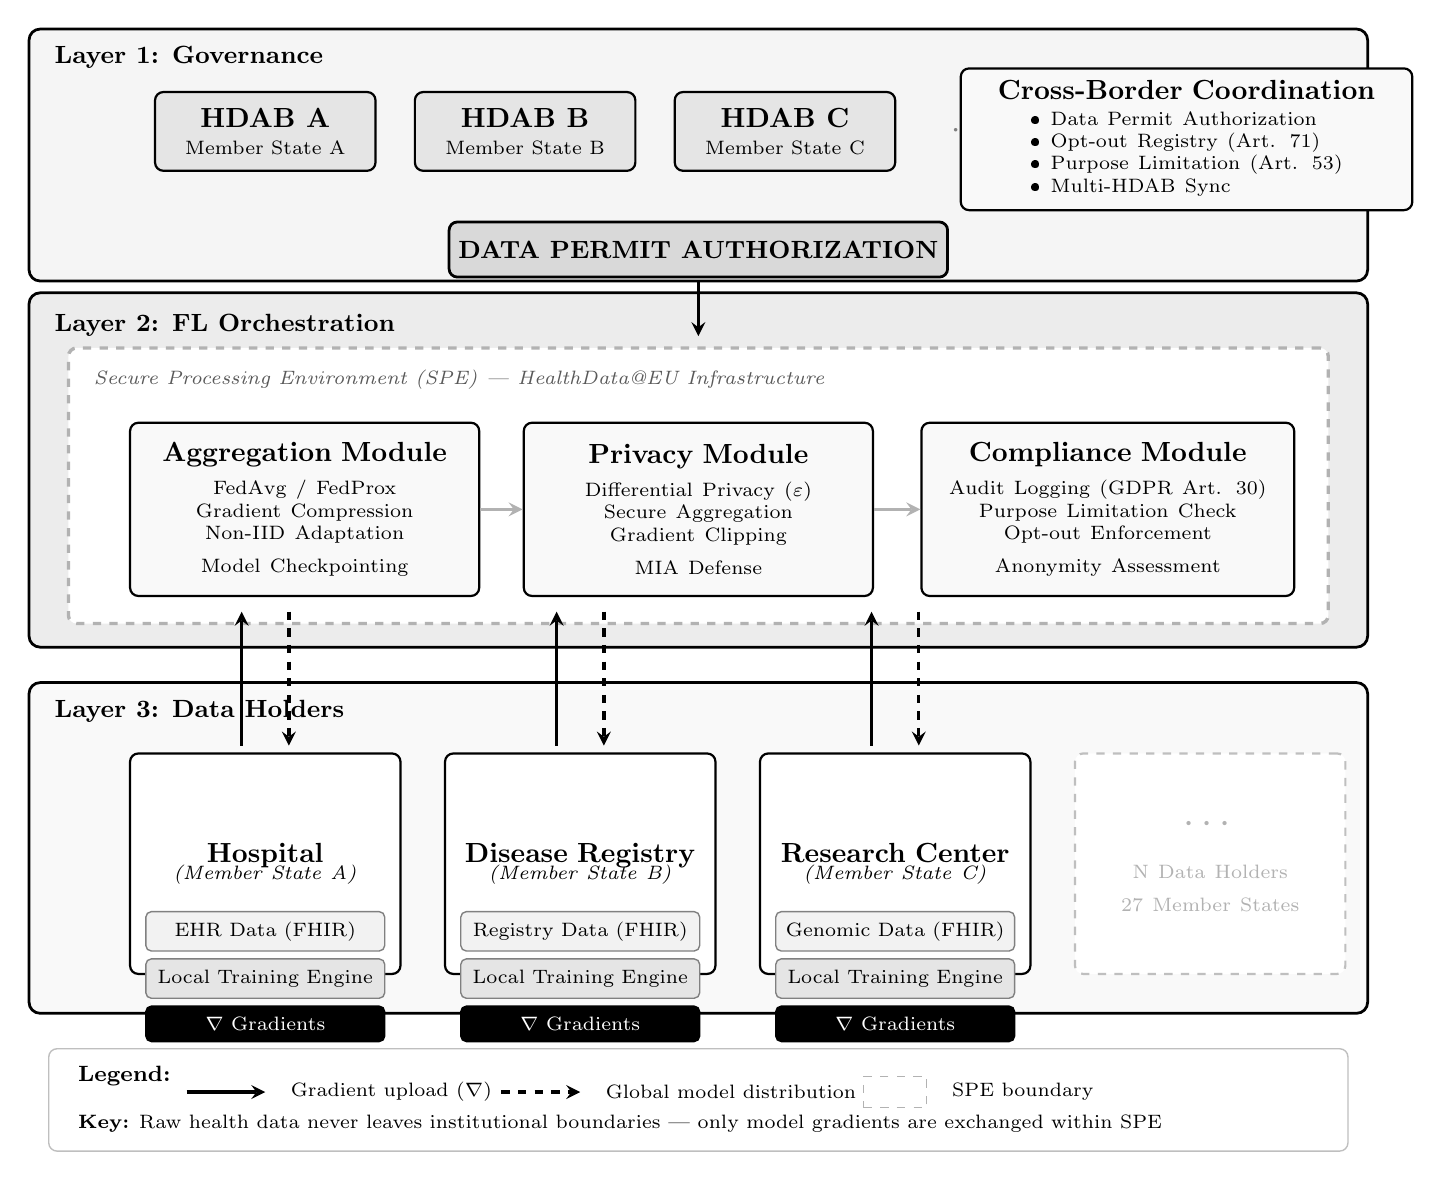
\begin{tikzpicture}[
    % Styles
    layer/.style={rectangle, rounded corners=4pt, minimum width=17cm, draw=black, line width=1pt},
    module/.style={rectangle, rounded corners=3pt, draw=black, line width=0.8pt, fill=white, minimum height=2.2cm, text width=4.2cm, align=center},
    hdab/.style={rectangle, rounded corners=3pt, draw=black, line width=0.8pt, fill=gray!20, minimum height=1cm, minimum width=2.8cm, align=center},
    dataholder/.style={rectangle, rounded corners=3pt, draw=black, line width=0.8pt, fill=white, minimum height=2.8cm, text width=3.2cm, align=center},
    databox/.style={rectangle, rounded corners=2pt, draw=gray, line width=0.5pt, fill=gray!10, minimum height=0.5cm, text width=2.8cm, align=center, font=\scriptsize},
    gradientbox/.style={rectangle, rounded corners=2pt, draw=black, line width=0.5pt, fill=black, minimum height=0.45cm, text width=2.8cm, align=center, font=\scriptsize\color{white}},
    arrow/.style={->, >=stealth, line width=1.2pt},
    dashedarrow/.style={->, >=stealth, line width=1.2pt, dashed},
    label/.style={font=\footnotesize},
    title/.style={font=\small\bfseries},
    subtitle/.style={font=\scriptsize\itshape, text=gray!70!black},
]

% ===== LAYER 1: GOVERNANCE =====
\node[layer, fill=gray!8, minimum height=3.2cm] (layer1) at (0, 8) {};
\node[title, anchor=north west] at (-8.3, 9.5) {Layer 1: Governance};

% HDABs
\node[hdab] (hdabA) at (-5.5, 8.3) {\textbf{HDAB A}\\[-2pt]\scriptsize Member State A};
\node[hdab] (hdabB) at (-2.2, 8.3) {\textbf{HDAB B}\\[-2pt]\scriptsize Member State B};
\node[hdab] (hdabC) at (1.1, 8.3) {\textbf{HDAB C}\\[-2pt]\scriptsize Member State C};
\node[font=\large, text=gray] at (3.5, 8.3) {$\cdots$};

% Coordination box
\node[module, minimum height=1.8cm, text width=5.5cm, fill=gray!5] (coord) at (6.2, 8.2) {
    \textbf{Cross-Border Coordination}\\[3pt]
    \scriptsize
    \begin{tabular}{@{}l@{}}
    • Data Permit Authorization\\
    • Opt-out Registry (Art. 71)\\
    • Purpose Limitation (Art. 53)\\
    • Multi-HDAB Sync
    \end{tabular}
};

% Data Permit box
\node[rectangle, rounded corners=3pt, draw=black, line width=1pt, fill=gray!30, minimum height=0.7cm, minimum width=5cm] (permit) at (0, 6.8) {\small\textbf{DATA PERMIT AUTHORIZATION}};

% ===== LAYER 2: FL ORCHESTRATION =====
\node[layer, fill=gray!15, minimum height=4.5cm] (layer2) at (0, 4) {};
\node[title, anchor=north west] at (-8.3, 6.1) {Layer 2: FL Orchestration};

% SPE boundary
\node[rectangle, rounded corners=3pt, draw=gray!60, line width=1.2pt, dashed, minimum width=16cm, minimum height=3.5cm, fill=white] (spe) at (0, 3.8) {};
\node[subtitle, anchor=north west] at (-7.8, 5.4) {Secure Processing Environment (SPE) — HealthData@EU Infrastructure};

% Modules
\node[module, fill=gray!5] (agg) at (-5, 3.5) {
    \textbf{Aggregation Module}\\[4pt]
    \scriptsize
    FedAvg / FedProx\\
    Gradient Compression\\
    Non-IID Adaptation\\
    Model Checkpointing
};

\node[module, fill=gray!5] (priv) at (0, 3.5) {
    \textbf{Privacy Module}\\[4pt]
    \scriptsize
    Differential Privacy ($\varepsilon$)\\
    Secure Aggregation\\
    Gradient Clipping\\
    MIA Defense
};

\node[module, fill=gray!5, text width=4.5cm] (comp) at (5.2, 3.5) {
    \textbf{Compliance Module}\\[4pt]
    \scriptsize
    Audit Logging (GDPR Art. 30)\\
    Purpose Limitation Check\\
    Opt-out Enforcement\\
    Anonymity Assessment
};

% Arrows between modules
\draw[arrow, gray!60] (agg.east) -- (priv.west);
\draw[arrow, gray!60] (priv.east) -- (comp.west);

% ===== LAYER 3: DATA HOLDERS =====
\node[layer, fill=gray!5, minimum height=4.2cm] (layer3) at (0, -0.8) {};
\node[title, anchor=north west] at (-8.3, 1.2) {Layer 3: Data Holders};

% Data holders
\node[dataholder] (hosp) at (-5.5, -1) {
    \textbf{Hospital}\\[-2pt]
    \scriptsize\textit{(Member State A)}\\[6pt]
};
\node[databox, anchor=north] at (-5.5, -1.6) {EHR Data (FHIR)};
\node[databox, anchor=north, fill=gray!20] at (-5.5, -2.2) {Local Training Engine};
\node[gradientbox, anchor=north] at (-5.5, -2.8) {$\nabla$ Gradients};

\node[dataholder] (reg) at (-1.5, -1) {
    \textbf{Disease Registry}\\[-2pt]
    \scriptsize\textit{(Member State B)}\\[6pt]
};
\node[databox, anchor=north] at (-1.5, -1.6) {Registry Data (FHIR)};
\node[databox, anchor=north, fill=gray!20] at (-1.5, -2.2) {Local Training Engine};
\node[gradientbox, anchor=north] at (-1.5, -2.8) {$\nabla$ Gradients};

\node[dataholder] (res) at (2.5, -1) {
    \textbf{Research Center}\\[-2pt]
    \scriptsize\textit{(Member State C)}\\[6pt]
};
\node[databox, anchor=north] at (2.5, -1.6) {Genomic Data (FHIR)};
\node[databox, anchor=north, fill=gray!20] at (2.5, -2.2) {Local Training Engine};
\node[gradientbox, anchor=north] at (2.5, -2.8) {$\nabla$ Gradients};

% More nodes indicator
\node[dataholder, draw=gray!50, dashed, text=gray!60] (more) at (6.5, -1) {
    \Large$\cdots$\\[8pt]
    \scriptsize N Data Holders\\
    27 Member States
};

% ===== DATA FLOW ARROWS =====
% Gradients up (solid)
\draw[arrow] (-5.8, 0.5) -- (-5.8, 2.2) node[midway, left, font=\tiny] {};
\draw[arrow] (-1.8, 0.5) -- (-1.8, 2.2);
\draw[arrow] (2.2, 0.5) -- (2.2, 2.2);

% Model down (dashed)
\draw[dashedarrow] (-5.2, 2.2) -- (-5.2, 0.5);
\draw[dashedarrow] (-1.2, 2.2) -- (-1.2, 0.5);
\draw[dashedarrow] (2.8, 2.2) -- (2.8, 0.5);

% Layer 1 to Layer 2
\draw[arrow] (0, 6.4) -- (0, 5.7);

% ===== LEGEND =====
\node[rectangle, rounded corners=3pt, draw=gray!50, line width=0.5pt, fill=white, minimum width=16.5cm, minimum height=1.3cm] at (0, -4) {};
\node[font=\footnotesize\bfseries, anchor=west] at (-8, -3.7) {Legend:};

% Gradient arrow
\draw[arrow] (-6.5, -3.9) -- (-5.5, -3.9);
\node[font=\scriptsize, anchor=west] at (-5.3, -3.9) {Gradient upload ($\nabla$)};

% Model arrow  
\draw[dashedarrow] (-2.5, -3.9) -- (-1.5, -3.9);
\node[font=\scriptsize, anchor=west] at (-1.3, -3.9) {Global model distribution};

% SPE
\node[rectangle, draw=gray!60, dashed, minimum width=0.8cm, minimum height=0.4cm] at (2.5, -3.9) {};
\node[font=\scriptsize, anchor=west] at (3.1, -3.9) {SPE boundary};

% Key principle
\node[font=\scriptsize, anchor=west] at (-8, -4.3) {\textbf{Key:} Raw health data never leaves institutional boundaries — only model gradients are exchanged within SPE};

\end{tikzpicture}
\caption{FL-EHDS three-layer compliance framework architecture. Layer~1 (Governance) integrates Health Data Access Bodies for cross-border data permit authorization and opt-out registry consultation per Article~71. Layer~2 (FL Orchestration) operates within a Secure Processing Environment, implementing gradient aggregation with FedAvg/FedProx, privacy protection via differential privacy and secure aggregation, and GDPR-compliant audit logging. Layer~3 (Data Holders) maintains raw data within institutional boundaries across 27 Member States; only gradients ($\nabla$) are transmitted upward while global model parameters flow downward.}
\label{fig:architecture}
\end{figure*}


\begin{figure*}[htbp]
\centering
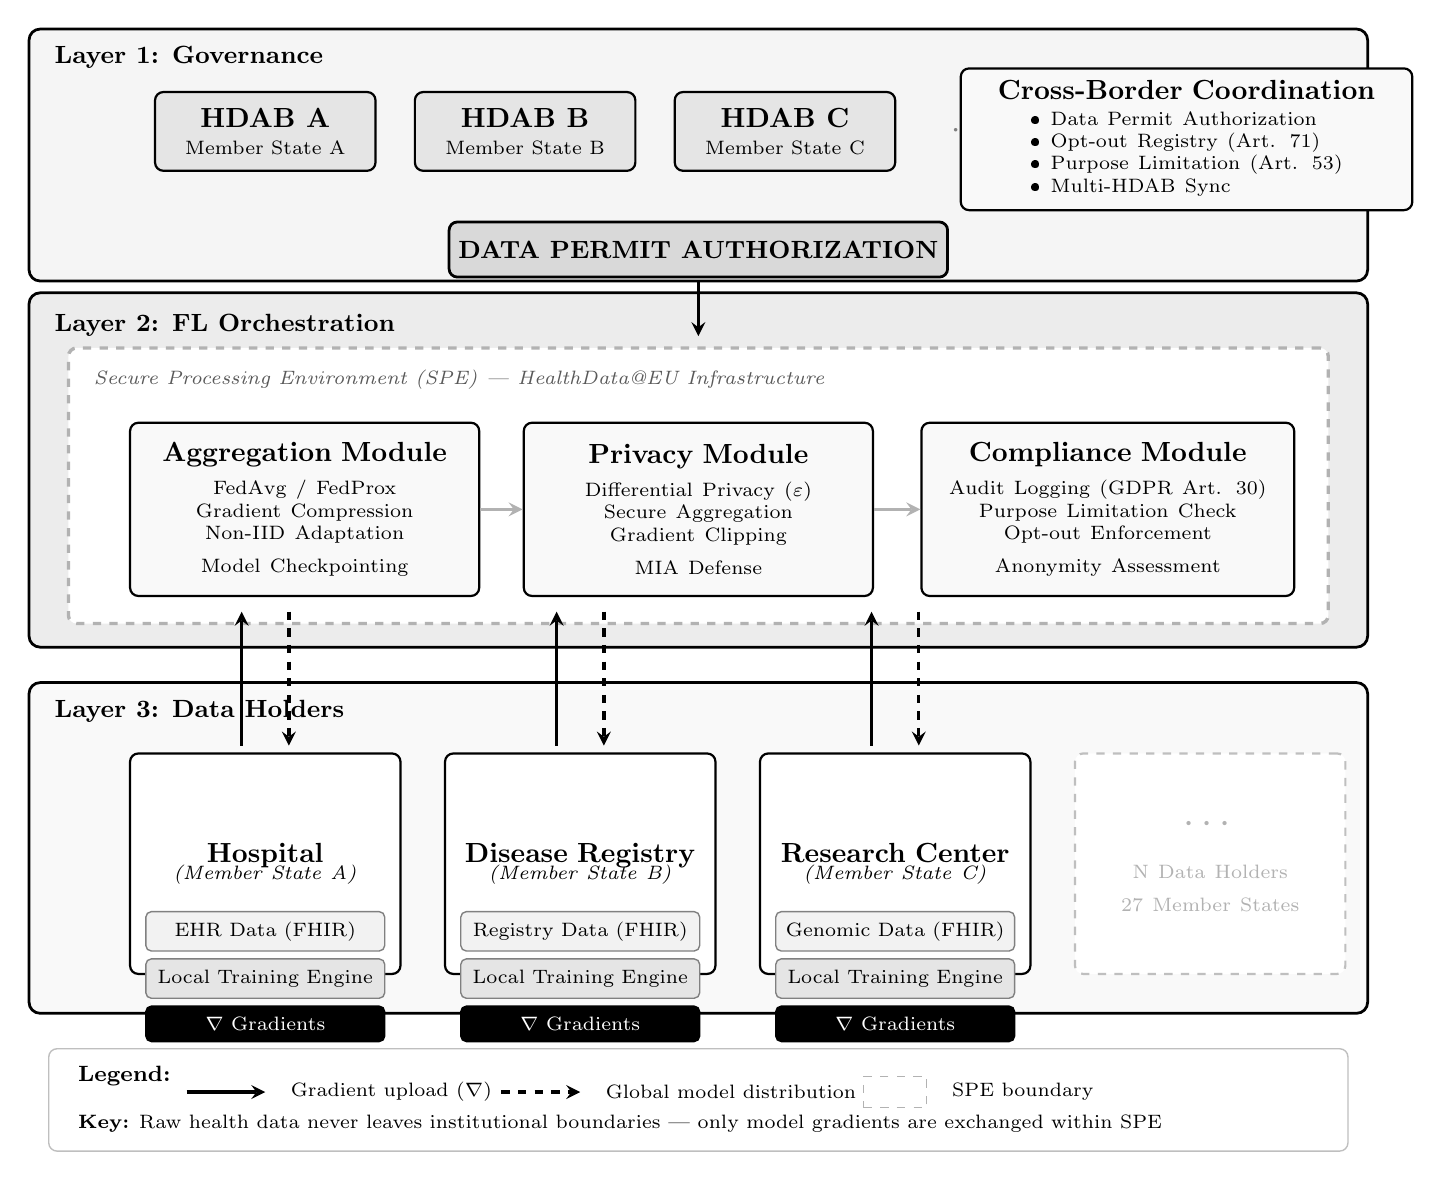
\begin{tikzpicture}[
    % Styles
    layer/.style={rectangle, rounded corners=4pt, minimum width=17cm, draw=black, line width=1pt},
    module/.style={rectangle, rounded corners=3pt, draw=black, line width=0.8pt, fill=white, minimum height=2.2cm, text width=4.2cm, align=center},
    hdab/.style={rectangle, rounded corners=3pt, draw=black, line width=0.8pt, fill=gray!20, minimum height=1cm, minimum width=2.8cm, align=center},
    dataholder/.style={rectangle, rounded corners=3pt, draw=black, line width=0.8pt, fill=white, minimum height=2.8cm, text width=3.2cm, align=center},
    databox/.style={rectangle, rounded corners=2pt, draw=gray, line width=0.5pt, fill=gray!10, minimum height=0.5cm, text width=2.8cm, align=center, font=\scriptsize},
    gradientbox/.style={rectangle, rounded corners=2pt, draw=black, line width=0.5pt, fill=black, minimum height=0.45cm, text width=2.8cm, align=center, font=\scriptsize\color{white}},
    arrow/.style={->, >=stealth, line width=1.2pt},
    dashedarrow/.style={->, >=stealth, line width=1.2pt, dashed},
    label/.style={font=\footnotesize},
    title/.style={font=\small\bfseries},
    subtitle/.style={font=\scriptsize\itshape, text=gray!70!black},
]

% ===== LAYER 1: GOVERNANCE =====
\node[layer, fill=gray!8, minimum height=3.2cm] (layer1) at (0, 8) {};
\node[title, anchor=north west] at (-8.3, 9.5) {Layer 1: Governance};

% HDABs
\node[hdab] (hdabA) at (-5.5, 8.3) {\textbf{HDAB A}\\[-2pt]\scriptsize Member State A};
\node[hdab] (hdabB) at (-2.2, 8.3) {\textbf{HDAB B}\\[-2pt]\scriptsize Member State B};
\node[hdab] (hdabC) at (1.1, 8.3) {\textbf{HDAB C}\\[-2pt]\scriptsize Member State C};
\node[font=\large, text=gray] at (3.5, 8.3) {$\cdots$};

% Coordination box
\node[module, minimum height=1.8cm, text width=5.5cm, fill=gray!5] (coord) at (6.2, 8.2) {
    \textbf{Cross-Border Coordination}\\[3pt]
    \scriptsize
    \begin{tabular}{@{}l@{}}
    • Data Permit Authorization\\
    • Opt-out Registry (Art. 71)\\
    • Purpose Limitation (Art. 53)\\
    • Multi-HDAB Sync
    \end{tabular}
};

% Data Permit box
\node[rectangle, rounded corners=3pt, draw=black, line width=1pt, fill=gray!30, minimum height=0.7cm, minimum width=5cm] (permit) at (0, 6.8) {\small\textbf{DATA PERMIT AUTHORIZATION}};

% ===== LAYER 2: FL ORCHESTRATION =====
\node[layer, fill=gray!15, minimum height=4.5cm] (layer2) at (0, 4) {};
\node[title, anchor=north west] at (-8.3, 6.1) {Layer 2: FL Orchestration};

% SPE boundary
\node[rectangle, rounded corners=3pt, draw=gray!60, line width=1.2pt, dashed, minimum width=16cm, minimum height=3.5cm, fill=white] (spe) at (0, 3.8) {};
\node[subtitle, anchor=north west] at (-7.8, 5.4) {Secure Processing Environment (SPE) — HealthData@EU Infrastructure};

% Modules
\node[module, fill=gray!5] (agg) at (-5, 3.5) {
    \textbf{Aggregation Module}\\[4pt]
    \scriptsize
    FedAvg / FedProx\\
    Gradient Compression\\
    Non-IID Adaptation\\
    Model Checkpointing
};

\node[module, fill=gray!5] (priv) at (0, 3.5) {
    \textbf{Privacy Module}\\[4pt]
    \scriptsize
    Differential Privacy ($\varepsilon$)\\
    Secure Aggregation\\
    Gradient Clipping\\
    MIA Defense
};

\node[module, fill=gray!5, text width=4.5cm] (comp) at (5.2, 3.5) {
    \textbf{Compliance Module}\\[4pt]
    \scriptsize
    Audit Logging (GDPR Art. 30)\\
    Purpose Limitation Check\\
    Opt-out Enforcement\\
    Anonymity Assessment
};

% Arrows between modules
\draw[arrow, gray!60] (agg.east) -- (priv.west);
\draw[arrow, gray!60] (priv.east) -- (comp.west);

% ===== LAYER 3: DATA HOLDERS =====
\node[layer, fill=gray!5, minimum height=4.2cm] (layer3) at (0, -0.8) {};
\node[title, anchor=north west] at (-8.3, 1.2) {Layer 3: Data Holders};

% Data holders
\node[dataholder] (hosp) at (-5.5, -1) {
    \textbf{Hospital}\\[-2pt]
    \scriptsize\textit{(Member State A)}\\[6pt]
};
\node[databox, anchor=north] at (-5.5, -1.6) {EHR Data (FHIR)};
\node[databox, anchor=north, fill=gray!20] at (-5.5, -2.2) {Local Training Engine};
\node[gradientbox, anchor=north] at (-5.5, -2.8) {$\nabla$ Gradients};

\node[dataholder] (reg) at (-1.5, -1) {
    \textbf{Disease Registry}\\[-2pt]
    \scriptsize\textit{(Member State B)}\\[6pt]
};
\node[databox, anchor=north] at (-1.5, -1.6) {Registry Data (FHIR)};
\node[databox, anchor=north, fill=gray!20] at (-1.5, -2.2) {Local Training Engine};
\node[gradientbox, anchor=north] at (-1.5, -2.8) {$\nabla$ Gradients};

\node[dataholder] (res) at (2.5, -1) {
    \textbf{Research Center}\\[-2pt]
    \scriptsize\textit{(Member State C)}\\[6pt]
};
\node[databox, anchor=north] at (2.5, -1.6) {Genomic Data (FHIR)};
\node[databox, anchor=north, fill=gray!20] at (2.5, -2.2) {Local Training Engine};
\node[gradientbox, anchor=north] at (2.5, -2.8) {$\nabla$ Gradients};

% More nodes indicator
\node[dataholder, draw=gray!50, dashed, text=gray!60] (more) at (6.5, -1) {
    \Large$\cdots$\\[8pt]
    \scriptsize N Data Holders\\
    27 Member States
};

% ===== DATA FLOW ARROWS =====
% Gradients up (solid)
\draw[arrow] (-5.8, 0.5) -- (-5.8, 2.2) node[midway, left, font=\tiny] {};
\draw[arrow] (-1.8, 0.5) -- (-1.8, 2.2);
\draw[arrow] (2.2, 0.5) -- (2.2, 2.2);

% Model down (dashed)
\draw[dashedarrow] (-5.2, 2.2) -- (-5.2, 0.5);
\draw[dashedarrow] (-1.2, 2.2) -- (-1.2, 0.5);
\draw[dashedarrow] (2.8, 2.2) -- (2.8, 0.5);

% Layer 1 to Layer 2
\draw[arrow] (0, 6.4) -- (0, 5.7);

% ===== LEGEND =====
\node[rectangle, rounded corners=3pt, draw=gray!50, line width=0.5pt, fill=white, minimum width=16.5cm, minimum height=1.3cm] at (0, -4) {};
\node[font=\footnotesize\bfseries, anchor=west] at (-8, -3.7) {Legend:};

% Gradient arrow
\draw[arrow] (-6.5, -3.9) -- (-5.5, -3.9);
\node[font=\scriptsize, anchor=west] at (-5.3, -3.9) {Gradient upload ($\nabla$)};

% Model arrow  
\draw[dashedarrow] (-2.5, -3.9) -- (-1.5, -3.9);
\node[font=\scriptsize, anchor=west] at (-1.3, -3.9) {Global model distribution};

% SPE
\node[rectangle, draw=gray!60, dashed, minimum width=0.8cm, minimum height=0.4cm] at (2.5, -3.9) {};
\node[font=\scriptsize, anchor=west] at (3.1, -3.9) {SPE boundary};

% Key principle
\node[font=\scriptsize, anchor=west] at (-8, -4.3) {\textbf{Key:} Raw health data never leaves institutional boundaries — only model gradients are exchanged within SPE};

\end{tikzpicture}
\caption{FL-EHDS three-layer compliance framework architecture. Layer~1 (Governance) integrates Health Data Access Bodies for cross-border data permit authorization and opt-out registry consultation per Article~71. Layer~2 (FL Orchestration) operates within a Secure Processing Environment, implementing gradient aggregation with FedAvg/FedProx, privacy protection via differential privacy and secure aggregation, and GDPR-compliant audit logging. Layer~3 (Data Holders) maintains raw data within institutional boundaries across 27 Member States; only gradients ($\nabla$) are transmitted upward while global model parameters flow downward.}
\label{fig:architecture}
\end{figure*}


\begin{figure*}[htbp]
\centering
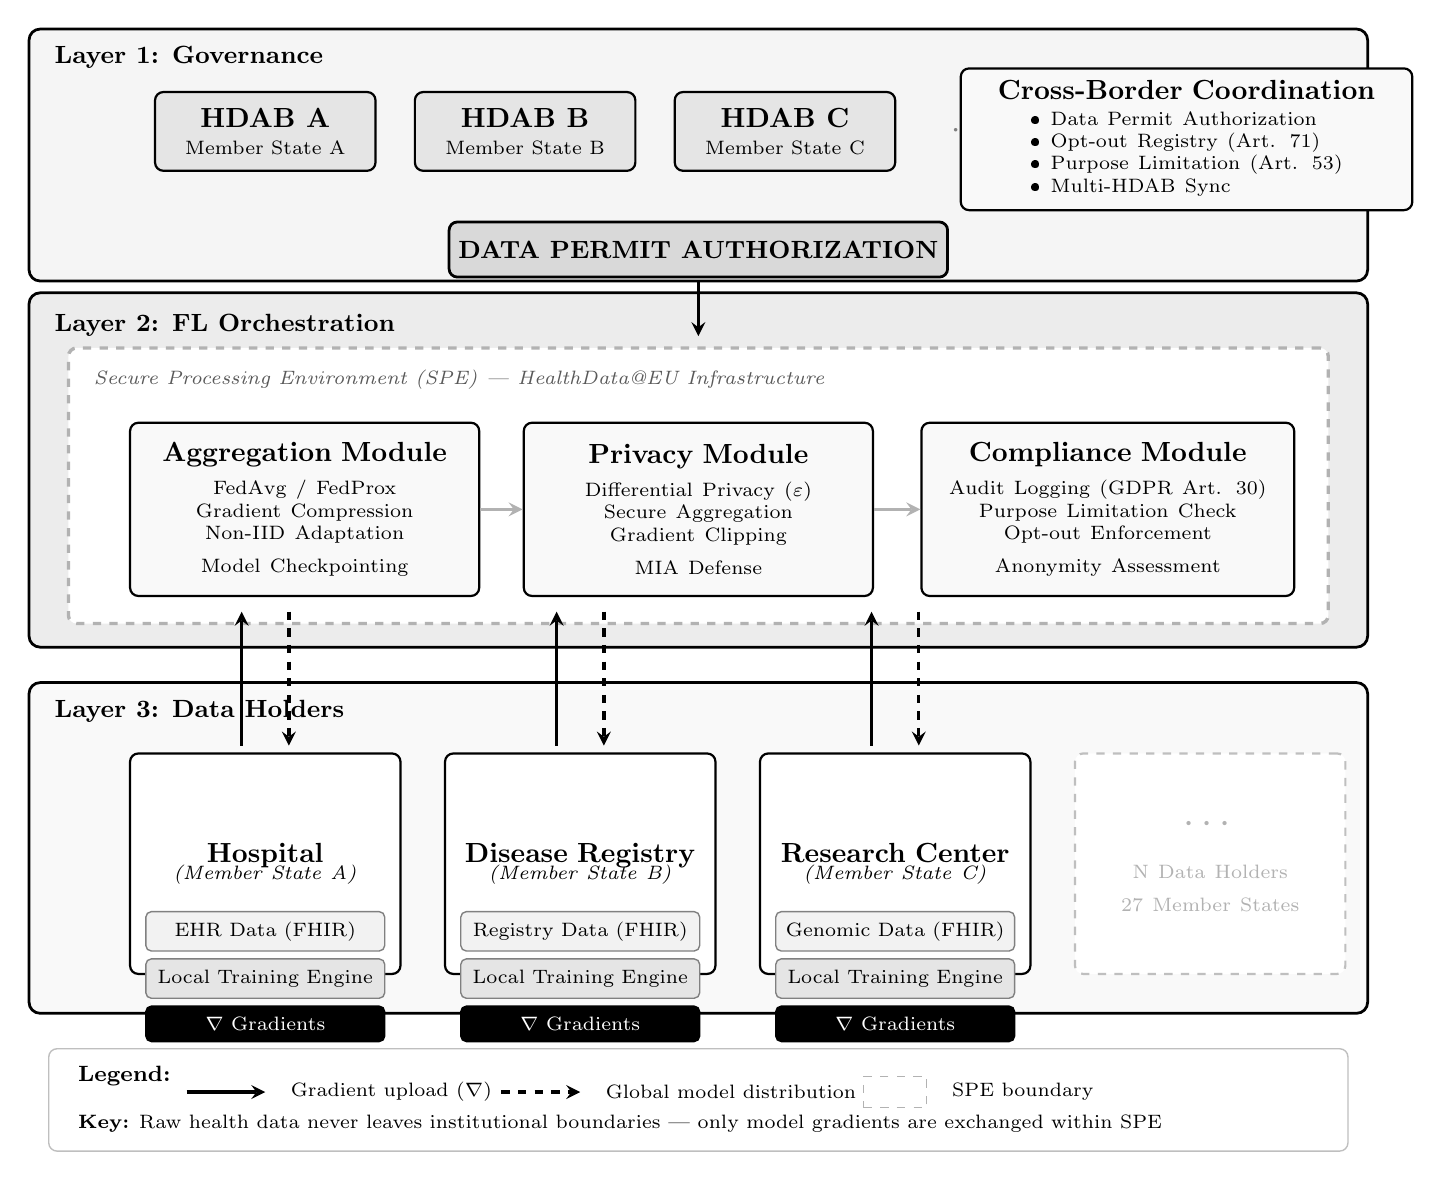
\begin{tikzpicture}[
    % Styles
    layer/.style={rectangle, rounded corners=4pt, minimum width=17cm, draw=black, line width=1pt},
    module/.style={rectangle, rounded corners=3pt, draw=black, line width=0.8pt, fill=white, minimum height=2.2cm, text width=4.2cm, align=center},
    hdab/.style={rectangle, rounded corners=3pt, draw=black, line width=0.8pt, fill=gray!20, minimum height=1cm, minimum width=2.8cm, align=center},
    dataholder/.style={rectangle, rounded corners=3pt, draw=black, line width=0.8pt, fill=white, minimum height=2.8cm, text width=3.2cm, align=center},
    databox/.style={rectangle, rounded corners=2pt, draw=gray, line width=0.5pt, fill=gray!10, minimum height=0.5cm, text width=2.8cm, align=center, font=\scriptsize},
    gradientbox/.style={rectangle, rounded corners=2pt, draw=black, line width=0.5pt, fill=black, minimum height=0.45cm, text width=2.8cm, align=center, font=\scriptsize\color{white}},
    arrow/.style={->, >=stealth, line width=1.2pt},
    dashedarrow/.style={->, >=stealth, line width=1.2pt, dashed},
    label/.style={font=\footnotesize},
    title/.style={font=\small\bfseries},
    subtitle/.style={font=\scriptsize\itshape, text=gray!70!black},
]

% ===== LAYER 1: GOVERNANCE =====
\node[layer, fill=gray!8, minimum height=3.2cm] (layer1) at (0, 8) {};
\node[title, anchor=north west] at (-8.3, 9.5) {Layer 1: Governance};

% HDABs
\node[hdab] (hdabA) at (-5.5, 8.3) {\textbf{HDAB A}\\[-2pt]\scriptsize Member State A};
\node[hdab] (hdabB) at (-2.2, 8.3) {\textbf{HDAB B}\\[-2pt]\scriptsize Member State B};
\node[hdab] (hdabC) at (1.1, 8.3) {\textbf{HDAB C}\\[-2pt]\scriptsize Member State C};
\node[font=\large, text=gray] at (3.5, 8.3) {$\cdots$};

% Coordination box
\node[module, minimum height=1.8cm, text width=5.5cm, fill=gray!5] (coord) at (6.2, 8.2) {
    \textbf{Cross-Border Coordination}\\[3pt]
    \scriptsize
    \begin{tabular}{@{}l@{}}
    • Data Permit Authorization\\
    • Opt-out Registry (Art. 71)\\
    • Purpose Limitation (Art. 53)\\
    • Multi-HDAB Sync
    \end{tabular}
};

% Data Permit box
\node[rectangle, rounded corners=3pt, draw=black, line width=1pt, fill=gray!30, minimum height=0.7cm, minimum width=5cm] (permit) at (0, 6.8) {\small\textbf{DATA PERMIT AUTHORIZATION}};

% ===== LAYER 2: FL ORCHESTRATION =====
\node[layer, fill=gray!15, minimum height=4.5cm] (layer2) at (0, 4) {};
\node[title, anchor=north west] at (-8.3, 6.1) {Layer 2: FL Orchestration};

% SPE boundary
\node[rectangle, rounded corners=3pt, draw=gray!60, line width=1.2pt, dashed, minimum width=16cm, minimum height=3.5cm, fill=white] (spe) at (0, 3.8) {};
\node[subtitle, anchor=north west] at (-7.8, 5.4) {Secure Processing Environment (SPE) — HealthData@EU Infrastructure};

% Modules
\node[module, fill=gray!5] (agg) at (-5, 3.5) {
    \textbf{Aggregation Module}\\[4pt]
    \scriptsize
    FedAvg / FedProx\\
    Gradient Compression\\
    Non-IID Adaptation\\
    Model Checkpointing
};

\node[module, fill=gray!5] (priv) at (0, 3.5) {
    \textbf{Privacy Module}\\[4pt]
    \scriptsize
    Differential Privacy ($\varepsilon$)\\
    Secure Aggregation\\
    Gradient Clipping\\
    MIA Defense
};

\node[module, fill=gray!5, text width=4.5cm] (comp) at (5.2, 3.5) {
    \textbf{Compliance Module}\\[4pt]
    \scriptsize
    Audit Logging (GDPR Art. 30)\\
    Purpose Limitation Check\\
    Opt-out Enforcement\\
    Anonymity Assessment
};

% Arrows between modules
\draw[arrow, gray!60] (agg.east) -- (priv.west);
\draw[arrow, gray!60] (priv.east) -- (comp.west);

% ===== LAYER 3: DATA HOLDERS =====
\node[layer, fill=gray!5, minimum height=4.2cm] (layer3) at (0, -0.8) {};
\node[title, anchor=north west] at (-8.3, 1.2) {Layer 3: Data Holders};

% Data holders
\node[dataholder] (hosp) at (-5.5, -1) {
    \textbf{Hospital}\\[-2pt]
    \scriptsize\textit{(Member State A)}\\[6pt]
};
\node[databox, anchor=north] at (-5.5, -1.6) {EHR Data (FHIR)};
\node[databox, anchor=north, fill=gray!20] at (-5.5, -2.2) {Local Training Engine};
\node[gradientbox, anchor=north] at (-5.5, -2.8) {$\nabla$ Gradients};

\node[dataholder] (reg) at (-1.5, -1) {
    \textbf{Disease Registry}\\[-2pt]
    \scriptsize\textit{(Member State B)}\\[6pt]
};
\node[databox, anchor=north] at (-1.5, -1.6) {Registry Data (FHIR)};
\node[databox, anchor=north, fill=gray!20] at (-1.5, -2.2) {Local Training Engine};
\node[gradientbox, anchor=north] at (-1.5, -2.8) {$\nabla$ Gradients};

\node[dataholder] (res) at (2.5, -1) {
    \textbf{Research Center}\\[-2pt]
    \scriptsize\textit{(Member State C)}\\[6pt]
};
\node[databox, anchor=north] at (2.5, -1.6) {Genomic Data (FHIR)};
\node[databox, anchor=north, fill=gray!20] at (2.5, -2.2) {Local Training Engine};
\node[gradientbox, anchor=north] at (2.5, -2.8) {$\nabla$ Gradients};

% More nodes indicator
\node[dataholder, draw=gray!50, dashed, text=gray!60] (more) at (6.5, -1) {
    \Large$\cdots$\\[8pt]
    \scriptsize N Data Holders\\
    27 Member States
};

% ===== DATA FLOW ARROWS =====
% Gradients up (solid)
\draw[arrow] (-5.8, 0.5) -- (-5.8, 2.2) node[midway, left, font=\tiny] {};
\draw[arrow] (-1.8, 0.5) -- (-1.8, 2.2);
\draw[arrow] (2.2, 0.5) -- (2.2, 2.2);

% Model down (dashed)
\draw[dashedarrow] (-5.2, 2.2) -- (-5.2, 0.5);
\draw[dashedarrow] (-1.2, 2.2) -- (-1.2, 0.5);
\draw[dashedarrow] (2.8, 2.2) -- (2.8, 0.5);

% Layer 1 to Layer 2
\draw[arrow] (0, 6.4) -- (0, 5.7);

% ===== LEGEND =====
\node[rectangle, rounded corners=3pt, draw=gray!50, line width=0.5pt, fill=white, minimum width=16.5cm, minimum height=1.3cm] at (0, -4) {};
\node[font=\footnotesize\bfseries, anchor=west] at (-8, -3.7) {Legend:};

% Gradient arrow
\draw[arrow] (-6.5, -3.9) -- (-5.5, -3.9);
\node[font=\scriptsize, anchor=west] at (-5.3, -3.9) {Gradient upload ($\nabla$)};

% Model arrow  
\draw[dashedarrow] (-2.5, -3.9) -- (-1.5, -3.9);
\node[font=\scriptsize, anchor=west] at (-1.3, -3.9) {Global model distribution};

% SPE
\node[rectangle, draw=gray!60, dashed, minimum width=0.8cm, minimum height=0.4cm] at (2.5, -3.9) {};
\node[font=\scriptsize, anchor=west] at (3.1, -3.9) {SPE boundary};

% Key principle
\node[font=\scriptsize, anchor=west] at (-8, -4.3) {\textbf{Key:} Raw health data never leaves institutional boundaries — only model gradients are exchanged within SPE};

\end{tikzpicture}
\caption{FL-EHDS three-layer compliance framework architecture. Layer~1 (Governance) integrates Health Data Access Bodies for cross-border data permit authorization and opt-out registry consultation per Article~71. Layer~2 (FL Orchestration) operates within a Secure Processing Environment, implementing gradient aggregation with FedAvg/FedProx, privacy protection via differential privacy and secure aggregation, and GDPR-compliant audit logging. Layer~3 (Data Holders) maintains raw data within institutional boundaries across 27 Member States; only gradients ($\nabla$) are transmitted upward while global model parameters flow downward.}
\label{fig:architecture}
\end{figure*}


\subsection{Layer 1: Governance Layer}

\textbf{HDAB Integration}: Standardized APIs enable automated data permit verification before FL training initiation. Multi-HDAB synchronization protocols coordinate cross-border studies involving multiple Member States, addressing the coordination complexity identified by Christiansen et al.~\cite{christiansen2025pilot}.

\textbf{Opt-out Registry}: National opt-out registries are consulted before each training round, ensuring Article 71 compliance. The framework implements granular opt-out checking at the record level while maintaining performance through caching mechanisms.

\textbf{Compliance Logging}: Comprehensive audit trails satisfy GDPR Article 30 requirements, documenting data access, processing purposes, and model outputs for regulatory inspection.

\subsection{Layer 2: FL Orchestration Layer}

\textbf{Aggregation Module}: The framework implements FedAvg~\cite{mcmahan2017communication} as the baseline aggregation algorithm, with FedProx~\cite{li2020federated} extensions for handling non-IID data distributions. Gradient compression techniques reduce communication overhead for cross-border model synchronization.

\textbf{Privacy Protection}: Differential privacy with configurable $\varepsilon$-budget provides formal privacy guarantees~\cite{dwork2014dp}. Gradient clipping bounds individual contribution magnitude, mitigating gradient inversion attacks~\cite{zhu2019deep}. Membership inference defense mechanisms prevent determination of training set membership~\cite{shokri2017membership}.

\textbf{Purpose Limitation}: Technical enforcement of permitted purposes (Article 53) through model output filtering and use-case validation, preventing scope creep beyond authorized analytics.

\subsection{Layer 3: Data Holder Layer}

\textbf{Adaptive Training Engine}: Resource-aware model partitioning addresses hardware heterogeneity (78\% barrier prevalence). The engine dynamically adjusts batch sizes, model complexity, and synchronization frequency based on local computational capabilities.

\textbf{FHIR Preprocessing}: Data normalization pipelines ensure interoperability across heterogeneous EHR systems. Only 34\% of European healthcare providers achieve full FHIR compliance~\cite{hussein2025interop}; the preprocessing module bridges format gaps through automated transformation.

\textbf{Secure Communication}: End-to-end encrypted gradient transmission ensures no raw data leaves institutional boundaries. Certificate-based authentication validates participant identity within the FL consortium.

% ============================================================================
% 4. EVIDENCE SYNTHESIS
% ============================================================================
\section{Evidence Synthesis}
\label{sec:evidence}

\subsection{Methodology}

We conducted a systematic review following PRISMA 2020 guidelines. Database searches (PubMed, IEEE Xplore, Scopus, Web of Science, arXiv) identified 847 records; after screening, 47 documents met inclusion criteria (publication 2022-2026, explicit FL/EHDS focus, peer-reviewed or recognized institutional origin). Quality was assessed using MMAT; confidence in findings using GRADE-CERQual. Full methodology is available from the corresponding author.

\subsection{Technical Barriers}

Table~\ref{tab:barriers} summarizes FL implementation barriers with prevalence, evidence sources, and FL-EHDS mitigation strategies.

\begin{table}[htbp]
\caption{FL Implementation Barriers for EHDS}
\label{tab:barriers}
\centering
\small
\begin{tabular}{p{2.0cm}cp{2.0cm}p{1.8cm}}
\toprule
\textbf{Barrier} & \textbf{Prev.} & \textbf{Evidence} & \textbf{Mitigation} \\
\midrule
Hardware heterogeneity & 78\% & Fr\"ohlich 2025 & Adaptive engine \\
Non-IID data & 67\% & Multiple & FedProx \\
Production gap & 23\% & Fr\"ohlich 2025 & Ref. implementation \\
FHIR compliance & 34\% & Hussein 2025 & Preprocessing \\
Communication cost & High & Bonawitz 2019 & Compression \\
\bottomrule
\end{tabular}
\end{table}

\textbf{GRADE-CERQual confidence}: MODERATE for technical barriers (limited by small number of rigorous evaluations in EHDS-specific contexts).

\subsection{Legal Uncertainties}

Three critical legal questions remain unresolved, creating compliance uncertainty that inhibits organizational FL adoption~\cite{quinn2024gdpr}:

\begin{enumerate}
    \item \textbf{Gradient data status}: Are model gradients ``personal data'' under GDPR? Gradient inversion attacks demonstrate potential re-identification~\cite{zhu2019deep}, but practical feasibility in production FL remains contested.
    \item \textbf{Model anonymity thresholds}: When does an aggregated model become sufficiently ``anonymous'' to escape GDPR scope? No established legal threshold exists.
    \item \textbf{Controller/processor allocation}: In multi-party FL, who bears data controller responsibilities---data holders, aggregation server operators, or model users?
\end{enumerate}

\textbf{GRADE-CERQual confidence}: MODERATE (coherent findings but rapidly evolving regulatory landscape).

\subsection{Organizational Barriers}

HDAB capacity shows significant variation across Member States. TEHDAS assessments~\cite{tehdas2024ready} reveal Nordic countries (Estonia, Finland, Denmark) demonstrate 2-3 year advantages in HDAB capacity-building, established health data infrastructure, and cross-border experience. Southern and Eastern European states face compressed timelines with limited baseline capacity, raising concerns about implementation equity.

\textbf{GRADE-CERQual confidence}: HIGH (consistent findings across multiple high-quality studies).

% ============================================================================
% 5. IMPLEMENTATION ROADMAP
% ============================================================================
\section{Implementation Roadmap}
\label{sec:roadmap}

Table~\ref{tab:roadmap} presents a phased implementation roadmap aligned with EHDS milestones.

\begin{table}[htbp]
\caption{FL-EHDS Implementation Roadmap}
\label{tab:roadmap}
\centering
\small
\begin{tabular}{llp{3.2cm}}
\toprule
\textbf{Phase} & \textbf{Timeline} & \textbf{Priority Actions} \\
\midrule
Foundation & 2025-26 & Reference implementation; multi-MS pilots \\
Clarification & 2027 & Delegated acts; legal guidance \\
Scaling & 2028-29 & Production deployment; capacity building \\
Operation & 2029-31 & Full cross-border analytics \\
\bottomrule
\end{tabular}
\end{table}

\subsection{Stakeholder-Specific Recommendations}

\textbf{EU Policymakers}: The March 2027 delegated acts represent a critical window. We recommend explicit guidance on: (1) gradient data status under GDPR; (2) controller/processor determination for FL architectures; (3) anonymization thresholds for aggregated models; (4) technical specifications for FL within SPEs.

\textbf{National Authorities}: Early investment in HDAB organizational capacity is essential. Staff training on FL evaluation, coordination protocols with other Member States, and stakeholder engagement with citizens about FL approaches should be prioritized. The 2-3 year Nordic advantage~\cite{tehdas2024ready} demonstrates that governance capacity may prove more constraining than technical infrastructure.

\textbf{Healthcare Organizations}: Preparation cannot wait for 2029. Organizations should: (1) accelerate FHIR compliance beyond the current 34\% baseline; (2) participate in HealthData@EU pilots to gain FL experience; (3) assess computational infrastructure for FL participation; (4) develop internal governance policies for responding to HDAB data access requests.

% ============================================================================
% 6. DISCUSSION
% ============================================================================
\section{Discussion}
\label{sec:discussion}

\subsection{Key Finding: Legal Uncertainties as Critical Blocker}

Our synthesis reveals that \textbf{legal uncertainties---not technical barriers---constitute the critical blocker} for FL adoption in EHDS contexts. While technical challenges (hardware heterogeneity, non-IID data, communication costs) are significant, they are tractable through known algorithmic solutions implemented in FL-EHDS Layer 2-3 components.

In contrast, unresolved regulatory questions create compliance uncertainty that healthcare organizations cannot navigate through engineering alone. Without clarification of gradient data status, organizations face potential GDPR violations regardless of technical privacy measures implemented. This finding aligns with van Drumpt et al.'s~\cite{vandrumpt2025pets} conclusion that governance frameworks are prerequisites, not alternatives, to technical solutions.

\subsection{Limitations}

This study has limitations informing interpretation. First, the FL/EHDS literature is rapidly evolving; publications after January 2026 are not captured. Second, most included studies analyze the newly-adopted regulation rather than actual implementation---empirical evidence on operational EHDS FL systems does not yet exist. Third, FL-EHDS framework validation remains conceptual; empirical evaluation through HealthData@EU pilot integration represents essential future work.

% ============================================================================
% 7. CONCLUSIONS
% ============================================================================
\section{Conclusions}
\label{sec:conclusions}

This paper presents FL-EHDS, a three-layer compliance framework bridging the technology-governance divide for cross-border health analytics under the European Health Data Space regulation.

Our systematic evidence synthesis reveals that \textbf{legal uncertainties---not technical barriers---constitute the critical blocker} for FL adoption in EHDS contexts. While technical challenges (hardware heterogeneity affecting 78\% of implementations, non-IID data impacting 67\% of models) are significant, they are tractable through known algorithmic solutions. The unresolved regulatory questions---gradient data status, model anonymity thresholds, controller allocation---create compliance uncertainty that discourages organizational adoption regardless of technical maturity.

The March 2027 delegated acts represent a critical window for resolution. Without explicit guidance on FL compliance, the 2029 secondary use deadline arrives with FL adoption inhibited by legal uncertainty rather than technical limitations. The 23\% production deployment rate documented in current literature~\cite{frohlich2025reality} will not improve through engineering advances alone.

\textbf{Future work} should prioritize: (1) empirical validation through HealthData@EU pilot integration; (2) citizen attitude studies examining FL acceptance and opt-out intentions; (3) economic sustainability modeling for HDAB operations; and (4) longitudinal tracking of implementation trajectories across diverse Member State contexts.

Only through coordinated action across EU policymakers, national authorities, and healthcare organizations can Federated Learning fulfill its potential as the enabling technology for privacy-preserving health analytics benefiting European citizens.

% ============================================================================
% ACKNOWLEDGMENTS
% ============================================================================
\section*{Acknowledgments}
The author thanks Prof.~Sadi Alawadi for supervision and guidance, and the TEHDAS Joint Action consortium for making preparatory materials publicly available.

% ============================================================================
% REFERENCES
% ============================================================================
\bibliographystyle{IEEEtran}

\begin{thebibliography}{00}

% === EHDS Regulation and Policy ===
\bibitem{eu2025ehds}
European Commission, ``Regulation (EU) 2025/327 on the European Health Data Space,'' \textit{Official Journal of the EU}, L 2025/327, Mar. 2025.

\bibitem{staunton2024ethical}
C. Staunton \textit{et al.}, ``Ethical and social reflections on the proposed European Health Data Space,'' \textit{Eur.~J.~Human Genetics}, vol.~32, no.~5, pp.~498--505, 2024.

\bibitem{quinn2024gdpr}
P. Quinn, E. Ellyne, and C. Yao, ``Will the GDPR restrain health data access bodies under the EHDS?'' \textit{Computer Law \& Security Review}, vol.~54, art.~105993, 2024.

\bibitem{tehdas2024ready}
TEHDAS Joint Action, ``Are EU member states ready for the European Health Data Space?'' \textit{Eur.~J.~Public Health}, vol.~34, no.~6, pp.~1102--1108, 2024.

% === EHDS Implementation Studies ===
\bibitem{frohlich2025reality}
H. Fr\"ohlich \textit{et al.}, ``Reality check: The aspirations of the EHDS amidst challenges in decentralized data analysis,'' \textit{J.~Med.~Internet Res.}, vol.~27, art.~e76491, 2025.

\bibitem{vandrumpt2025pets}
S. van Drumpt \textit{et al.}, ``Secondary use under the European Health Data Space: Setting the scene and towards a research agenda on privacy-enhancing technologies,'' \textit{Frontiers in Digital Health}, vol.~7, art.~1602101, 2025.

\bibitem{hussein2025interop}
R. Hussein \textit{et al.}, ``Interoperability framework of the EHDS for secondary use: Interactive EIF-based standards compliance toolkit,'' \textit{J.~Med.~Internet Res.}, vol.~27, art.~e69813, 2025.

\bibitem{forster2025journeys}
R. Forster \textit{et al.}, ``User journeys in cross-European secondary use of health data: Insights ahead of the EHDS,'' \textit{Eur.~J.~Public Health}, vol.~35, Suppl.~3, pp.~iii18--iii24, 2025.

\bibitem{svingel2025hdab}
L. Svingel \textit{et al.}, ``Shaping the future EHDS: Recommendations for implementation of Health Data Access Bodies,'' \textit{Eur.~J.~Public Health}, vol.~35, Suppl.~3, pp.~iii32--iii38, 2025.

\bibitem{christiansen2025pilot}
C. Christiansen \textit{et al.}, ``Piloting an infrastructure for secondary use of health data: Learnings from the HealthData@EU Pilot,'' \textit{Eur.~J.~Public Health}, vol.~35, Suppl.~3, pp.~iii3--iii4, 2025.

\bibitem{ganna2024boost}
A. Ganna, E. Ingelsson, and D. Posthuma, ``The European Health Data Space can be a boost for research beyond borders,'' \textit{Nature Medicine}, vol.~30, pp.~3053--3056, 2024.

% === Federated Learning Foundations ===
\bibitem{mcmahan2017communication}
B. McMahan \textit{et al.}, ``Communication-efficient learning of deep networks from decentralized data,'' in \textit{Proc. AISTATS}, pp.~1273--1282, 2017.

\bibitem{li2020federated}
T. Li \textit{et al.}, ``Federated optimization in heterogeneous networks,'' in \textit{Proc. MLSys}, vol.~2, pp.~429--450, 2020.

\bibitem{kairouz2021advances}
P. Kairouz \textit{et al.}, ``Advances and open problems in federated learning,'' \textit{Found.~Trends Mach.~Learn.}, vol.~14, no.~1--2, pp.~1--210, 2021.

\bibitem{rieke2020future}
N. Rieke \textit{et al.}, ``The future of digital health with federated learning,'' \textit{npj Digital Medicine}, vol.~3, art.~119, 2020.

\bibitem{bonawitz2019scale}
K. Bonawitz \textit{et al.}, ``Towards federated learning at scale: A system design,'' in \textit{Proc. MLSys}, pp.~374--388, 2019.

% === FL Systematic Reviews ===
\bibitem{teo2024systematic}
Z. L. Teo \textit{et al.}, ``Federated machine learning in healthcare: A systematic review on clinical applications and technical architecture,'' \textit{Cell Reports Medicine}, vol.~5, no.~2, art.~101419, 2024.

\bibitem{peng2024systematic}
L. Peng \textit{et al.}, ``Federated machine learning in healthcare: A systematic review on clinical applications and technical architecture,'' \textit{Comput.~Methods Programs Biomed.}, vol.~247, art.~108066, 2024.

% === Privacy and Security ===
\bibitem{zhu2019deep}
L. Zhu, Z. Liu, and S. Han, ``Deep leakage from gradients,'' in \textit{Proc. NeurIPS}, vol.~32, pp.~14774--14784, 2019.

\bibitem{shokri2017membership}
R. Shokri \textit{et al.}, ``Membership inference attacks against machine learning models,'' in \textit{Proc. IEEE S\&P}, pp.~3--18, 2017.

\bibitem{dwork2014dp}
C. Dwork and A. Roth, ``The algorithmic foundations of differential privacy,'' \textit{Found.~Trends Theor.~Comput.~Sci.}, vol.~9, no.~3--4, pp.~211--407, 2014.

\bibitem{abadi2016deep}
M. Abadi \textit{et al.}, ``Deep learning with differential privacy,'' in \textit{Proc. ACM CCS}, pp.~308--318, 2016.

\end{thebibliography}

\end{document}
